\documentclass{article}
\usepackage{blindtext}
\usepackage{hyperref}
\usepackage{graphicx}
\usepackage[letterpaper,top=3cm,bottom=3cm,left=3cm,right=3cm,marginparwidth=1.75cm]{geometry}
\usepackage{enumitem}
\usepackage{subfig}
\usepackage[italian]{babel}
\begin{document}

\begin{titlepage}
    \begin{center}

        \textbf{\LARGE Università degli studi di salerno}

        \vspace{0.5cm}
        
        
\includegraphics[width=0.5\textwidth]{unisa.png} 
        
        \vspace{0.3cm}
                
        \large Dipartimento di Informatica
        
        \vspace{3cm}
        
        \Huge \textbf{Sapore DiVino}
        
        \vspace{0.2cm}
        
        \large Progetto realizzato per il corso di \textit {Fondamenti di Intelligenza Artificiale}
        
        \vspace{3.0cm}
        
        \large \textbf{Progettista:} Fabio Sessa \\
        \large \textbf{Matricola:} 0512114634 \\
        \vspace{1.6cm}
        2023/2024
        
        \vspace{2cm}
    \end{center}
        \newpage
        \tableofcontents

        \newpage
        \section{Introduzione}
            L'universo del vino è un affascinante viaggio sensoriale che coinvolge tutti i nostri sensi, dalla vista al gusto, fino all'olfatto. Gli appassionati di vino apprezzano non solo la bevanda in sé, ma anche la complessità e la raffinatezza che si celano dietro ogni bottiglia. \\
            Per la realizzazione di questo progetto presente nella mia \href{https://github.com/bafiuss/SaporeDiVino.git}{repository GitHub}, sono presenti tutti i file relativi alla documentazione, presentazione e codice. 

        
        \subsection{Obiettivi}
            Durante realizzazione di questo progetto per il corso Fondamenti di Intelligenza Artificiale, mi sono cimentato in un problema comune di classificazione per quanto riguarda il Machine Learning; riguardo questo campo ho sempre avuto un interesse particolare ma prima di questa esperienza non né ho mai avuto un approccio effettivo. \\
            Le tematiche che andremo a toccare e gli obiettivi principali sono:
             \begin{itemize}
                \item analisi dettagliata di un \href{https://www.kaggle.com/datasets/uciml/red-wine-quality-cortez-et-al-2009}{dataset di vini rossi};
                \item l'identificazione di feature associate ai vini;
                \item l'implementazione di un modello di apprendimento in grado di classificare in modo affidabile la qualità di vini sufficienti e insufficienti.
            \end{itemize}
            
        \subsection{Specifica PEAS}
        \begin{itemize}
            \item \textbf{Performance}, ovvero le misure di prestazione adottate per valutare l’operato di un agente. Nel mio caso accuracy, recall, precision, F1 score e MCC;
            \item \textbf{Environment}, ovvero gli elementi che formano l’ambiente. Nel mio caso sarà costituito dall'elenco dei vini rossi;
            \item \textbf{Actuators}, ovvero gli attuatori disponibili all’agente per intraprendere le azioni. Nel mio caso sarà l'utilizzo di un algoritmo di classificazione
            \item \textbf{Sensors}, ovvero i sensori attraverso i quali l'agente riceve gli input percettivi. Nel mio caso l'agente va ad acquisire i dati utili per classificare la qualità di un vino.
        \end{itemize}

        \newpage
        \subsection{Caratteristiche dell'ambiente}
        L'ambiente è:
        \begin{itemize}
            \item \textbf{Single-agent}.
            \item \textbf{Parzialmente osservabile}: non si ha accesso a tutte le informazioni complete relative ai vini.
            \item \textbf{Stocastico}: le qualità dei vini possono essere influenzate da fattori  difficilmente prevedibili o che presentano una certa variabilità.
            \item \textbf{Sequenziale}: ... .
            \item \textbf{Dinamico}: la qualità può variare da vino in vino.
            \item \textbf{Discreto}: le variabili assumono valori in un limitato intervallo; alcune, invece, assumono valori distinti e separati.
        \end{itemize}

        \subsection{Analisi del problema}
        Il progetto affronta, dunque, quello che un problema di \textbf{apprendimento supervisionato} basato sulla costruzione di un modello di Machine Learning. 
        Inoltre, la classificazione che andremo ad utilizzare sarà di tipo \textbf{binario}, dato che puo assumere valori 0 e 1 (1 se il vino ha una qualità sufficiente, 0 se il vino ha una qualità insufficiente) \\
        Le tecnologie e gli strumenti che ho utilizzato sono i seguenti:
        \begin{itemize}
            \item \textbf{Visual Studio Code} come IDE;
            \item \textbf{Python} come linguaggio;
            \item \textbf{GitHub} per il versionamento;
            \item \textbf{JupyterNotebook} all’interno dell’IDE;
            \item \textbf{Overleaf} per la scrittura della documentazione;
            \item \textbf{Canva} per la realizzazione della presentazione.
        \end{itemize}

        \newpage
        \section{Data Understanding}
        La fase di Data Understanding implica un esame più attento dei dati disponibili per il data mining. Questo passaggio è di fondamentale importanza per evitare problemi imprevisti durante la fase successiva di Data Preparation, che è in genere la parte più lunga di un progetto. \\
        Inoltre questa fase è composta da:
        \begin{itemize}
            \item \textbf{Data Collection};
            \item \textbf{Data Description};
            \item \textbf{Data Quality};
        \end{itemize}

         \subsection{Data Collection}
         In linea generale, la fase di Data Collection è il processo di raccolta, misurazione e analisi delle informazioni provenienti da innumerevoli fonti diverse. Dopo varie ricerche online del giusto dataset, ho deciso di scegliere un dataset presente su Kaggle,  una piattaforma online dedicata alle competizioni di data science, machine learning e analisi dei dati. Il riferimento al dataset lo si può trovare al seguente \href{https://www.kaggle.com/datasets/uciml/red-wine-quality-cortez-et-al-2009}{link}.

         \subsection{Data Description}
         Il dataset scelto è un elenco di vini e per gli appassionati più interessati, si tratta di vini rossi provenienti dal Portogallo. Possiamo trovare la bellezza di ben 1599 righe e 12 colonne. L'ultima colonna, ovvero 'quality', è quella che utilizzeremo per stabilire se la qualità di un vino è sufficiente(qualità del vino \( < \)=6) oppure insufficiente (qualità del vino \( > \)6). \\
         Non essendo un esperto ed appassionato di chimica, ho dovuto studiare più nel dettaglio quelle che sono le caratteristiche che formano il dataset. Di seguito vi è una descrizione generale e sintetica delle caratteristiche:
         \begin{enumerate}
            \item \textbf{Fixed acidity}: si riferisce alla quantità di acidi presenti nel vino;
            \item \textbf{Volatile acidity}: si riferisce alla presenza di acidi volatili, ovvero composti chimici acidi che possono evaporare facilmente in forma di gas;
            \item \textbf{Citric acid}: elemento che può contribuire al profilo di acidità totale del vino;
            \item \textbf{Residual sugar}: si riferisce agli zuccheri lasciati non fermentati in un vino finito;
            \item \textbf{Chlorides}: quantità di sale nel vino;
            \item \textbf{Free sulfur dioxide}: sono i sulfuri disponibili a reagire e quindi presentano proprietà sia germicide che antiossidanti;
            \item \textbf{Total sulfur dioxide}: rappresenta la somma delle quantità di anidride solforosa libera e combinata presenti nel vino;
            \item \textbf{Density}: si riferisce alla quantità di materia presente in una determinata quantità di liquido;
            \item \textbf{pH}: descrive quanto è acido o basico un vino su una scala da 0 (molto acido) a 14 (molto basico);
            \item \textbf{Sulphates}: si riferiscono all'anidride solforosa (SO2), un composto chimico usato come conservante;
            \item \textbf{Alcohol}: percentuale di alcol del vino;
            \item \textbf{Quality}: variabile di output (sulla base dei dati sensoriali, punteggio compreso tra 3 e 8). 
         \end{enumerate}

        \newpage
        Un altro strumento molto utile per capire meglio la distribuzione dei dati è l'uso dei grafici, più in particolare degli istogrammi. Di seguito vi è una rappresentazione grafica riguardante le frequenze di ogni qualità della quantità di alcol presente nei vini suddivisi sempre per qualità

        \begin{figure}[ht]
            \centering
            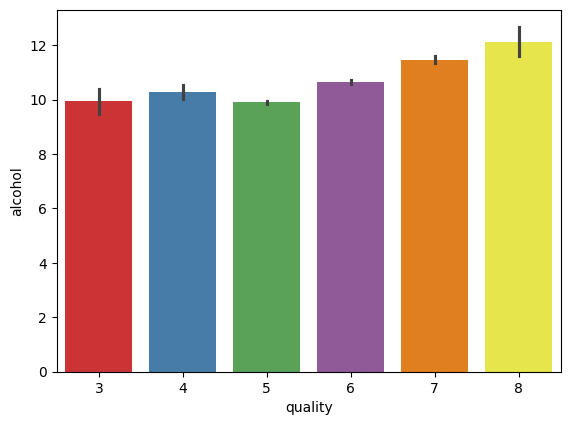
\includegraphics[width=0.5\linewidth]{barPlot-alcohol.png}
            \caption{ quantità di alcol nei vini suddivisi per qualità}
            \label{fig:enter-label}
        \end{figure}

        Come possiamo notare dal grafico, la distribuzione di alcol nei vini aumenta con l'aumentare della qualità di quest'ultimi.
        
        Il grafico seguente, invece, rappresenta le frequenze di vini di ogni qualità
        
        \begin{figure}[ht]
            \centering
            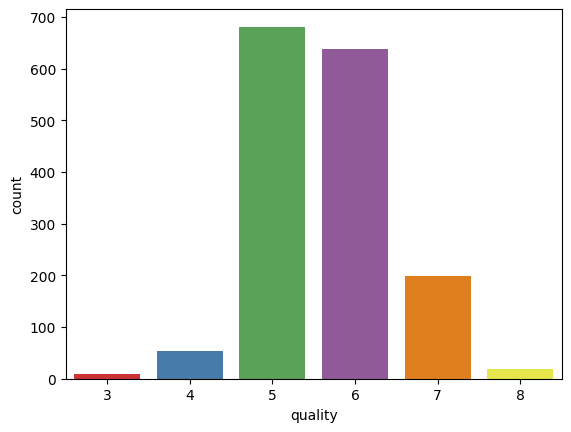
\includegraphics[width=0.5\linewidth]{countPlot-quality.png}
            \caption{ frequenze delle qualità}
            \label{fig:enter-label}
        \end{figure}

        Salta subito all'occhio che il grafico è meno distribuito rispetto al precedente, ma possiamo trarre alcune conclusioni, come ad esempio la moda della qualità che è rappresentata dal valore 5; inoltre la quantità di vini con qualità ottima/eccellente è molto scarsa.

        \newpage
        \subsection{Data Quality}
        In questa fase vado ad analizzare la qualità dei miei dati.
        L'obiettivo primario, ricordiamo, è la corretta classificazione della qualità di un vino e classificarla come sufficiente (qualità \( >\)=6) o come insufficiente (qualità \( <\)6). Non mi resta altro che suddividere la qualità in queste due categorie e con l'aiuto del grafico possiamo studiare al meglio la situazione

        \begin{figure}[ht]
            \centering
            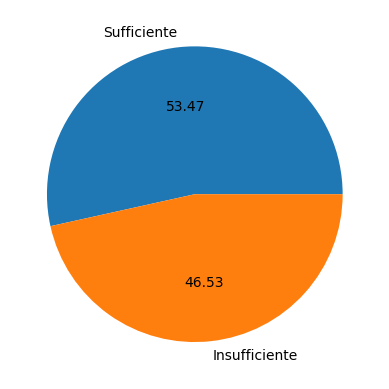
\includegraphics[width=0.5\linewidth]{pie-quality.png}
            \caption{  percentuali di frequenza delle classi}
            \label{fig:enter-label}
        \end{figure}

        Dal grafico possiamo notare che i vini con una qualità sufficiente sono molti di più rispetto ai vini con una qualità insufficiente.        
        Inoltre, dobbiamo gestire anche il problema dello sbilanciamento, ma questa tematica sarà affrontata più avanti nella fase del Data Balancing.

        \section{Data Preparation}
        La fase di Data Preparation ha lo scopo di eseguire una serie di attività volte a raccogliere, pulire, trasformare e organizzare i dati in modo che siano pronti per l'analisi o per l'addestramento di modelli di machine learning.\\
        Tale fase è suddivisa in diverse fasi, eseguite in modo cronologico:
        \begin{itemize}
            \item Data Cleaning
            \item Feature Scaling
            \item Feature Selection
            \item Data Balancing
        \end{itemize}

        \subsection{Data Cleaning}
        La fase di Data Cleaning  è progettata per identificare e correggere gli errori, le inconsistenze e le irregolarità nei dati raccolti. Alcuni esempi possono essere la presenza di dati mancanti in alcune righe, la presenza di intere colonne con valore nullo oppure la presenza di duplicati all'interno del dataset. Nel mio caso, non avendo valori nulli, ho dovuto affrontare solo il problema dei duplicati (ben 240) che non ho esitato a rimuovere, dato che potrebbero creare problemi nella classificazione binaria. 

        \newpage
        \subsection{Feature Scaling}
        La fase di Feature Scaling consiste nel trasformare le variabili del dataset in modo che siano tutte su una scala comune. Il motivo principale dietro tale fase è che molte tecniche di Machine Learning possono essere influenzate negativamente da differenze nelle scale delle variabili. \\Le due tecniche che abbiamo studiato sono: min-max normalization e z-score normalization; tra le due ho optato per la tecnica del \textbf{min-max normalization}, dove l'obiettivo di questa tecnica è trasformare le variabili in modo che abbiano valori compresi tra un certo intervallo, di solito tra 0 e 1. \\
        Effettuata l'operazione di normalizzazione, posso passare alla fase successiva, ossia la Feature Selection.

        \subsection{Feature Selection}
        Tale fase è un processo che coinvolge la scelta delle variabili (o caratteristiche) più rilevanti da utilizzare per costruire un modello predittivo o analizzare i dati. In generale, le "feature" si riferiscono alle variabili o attributi che vengono utilizzati per descrivere gli esempi nei dati. \\
        Per ottenere una panoramica generale delle correlazioni tra le varie caratteristiche, mi sono aiutato con quella che vien chiamata \textbf{matrice di correlazione}: è una matrice quadrata in cui ogni cella rappresenta la correlazione tra due variabili. Di seguito una guida per leggere al meglio una matrice di correlaizione:
        
        \begin{itemize}
            \item la diagonale principale della matrice contiene sempre valori di correlazione 1, poiché una variabile è sempre perfettamente correlata con se stessa.
            \item le celle più scure o più chiare indicano correlazioni più forti o più deboli, rispettivamente.
            \item le variabili sono fortemente correlate tra loro se hanno valori vicini a 1 o -1, mentre hanno una bassa correlazione se hanno valori vicini a 0.
        \end{itemize}

        \begin{figure}[ht]
            \centering
            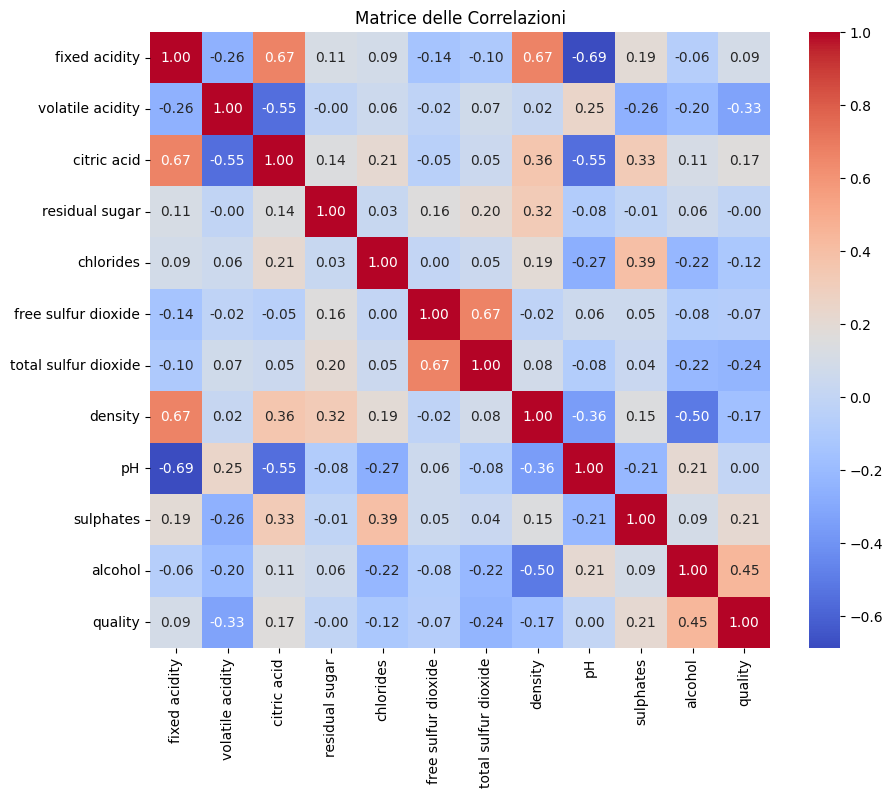
\includegraphics[width=0.6\linewidth]{correlation-matrix.png}
            \caption{  matrice delle correlazioni}
            \label{fig:enter-label}
        \end{figure}

        \newpage
        La matrice di correlazione appena calcolata presenta il problema di \textbf{multicollinearità}, ovvero in cui due o più variabili indipendenti sono fortemente correlate tra loro; infatti:
        \begin{itemize}
            \item \textbf{free-sulfur-dioxide} e \textbf{total-sulfur-dioxide} sono ben correlate positivamente (0.67);
            \item\textbf{pH} e \textbf{fixed-acidity} sono altamente correlate negativamente (-0.69).
        \end{itemize}

        \subsection{Data Balancing}
        L'obiettivo del Data Balancing è affrontare situazioni in cui le classi di un insieme di dati non sono rappresentate in modo uniforme, cioè alcune classi possono essere sovrarappresentate rispetto ad altre.\\
        Come enunciato in precedenza, il mio dataset presenta una classe maggioritaria di vini con qualità almeno sufficiente rispetto a vini con qualità insufficiente. Le tecinche che ho studiato durante il corso sono:
        \begin{itemize}
            \item la tecnica dell'\textbf{under-sampling}: eliminare casualmente le istanze della classe di maggioranza;
            \item la tecnica dell'\textbf{over-sampling}: eliminare casualmente le istanze della classe di minoranza.
        \end{itemize}
        Entrambe le tecniche vanno usate nel giusto modo e trattate con particolare attenzione.\\ Per bilanciare il dataset e per evitare di andare ad effettuare duplicazioni che potrebbero causare overfitting (quando un modello di Machine Learning si adatta troppo bene ai dati di addestramento) con l'utilizzo dell'over-sampling, ho preferito utilizzare la tecnica dell'\textbf{under-sampling}. \\ La rimozione delle istanze della classe maggioritaria è stata effettuata tramite \textit{RandomUndersampler}, uno strumento contenuto nella libreria sklearn.
        \\ Di seguito vi è il dataset prima dell'utilizzo dello strumento:
        \begin{itemize}
            \item Vini che hanno una qualità insufficiente: 640
            \item Vini che hanno una qualità almeno sufficiente: 719
        \end{itemize}
        Dopo l'utilizzo dello strumento:
        \begin{itemize}
            \item Vini che hanno una qualità insufficiente: 640
            \item Vini che hanno una qualità almeno sufficiente: 640
        \end{itemize}
        Notiamo che l'operazione di bilanciamento è stata eseguita con successo.
        \newpage
        \section{Data Modeling}
        Dopo aver effettuato le varie operazioni riguardanti la Data Preparation, possiamo affrontare quella che è la fase del Data Modeling. Tale fase, infatti, comprende diverse attività cruciali che si sulla rappresentazione dei dati in modo che possano essere utilizzati efficacemente dal modello di Machine Learning. \\
        Prima di proseguire, mi sono adoperato ad effettuare la divisione del dataset e affrontare il problema del data leakage (fuga di dati). La divisione del dataset è avvenuta in due gruppi: il 70\% del è dedicato all'addestramento (\textbf{training set}) e il 30\% è dedicato al testing (\textbf{test set}).

        \subsection{Scelta dei classificatori}
        I classificatori in Machine Learning sono algoritmi o modelli che vengono addestrati per assegnare etichette o categorie a dati non etichettati sulla base delle informazioni apprese da dati precedentemente etichettati durante la fase di addestramento. \\
        Nel mio caso, l'intero progetto è strutturato su un problema di classificazione binaria, dove la variabile target può assumere può assumere il valore 0 se la qualità è insufficiente, oppure il valore 1 se la qualità è almeno sufficiente. Tra i classificatori studiati durante il corso, possiamo trovare l'algoritmo di \textbf{Naive Bayes} (e relative varianti) e i \textbf{decision tree} (alberi decisionali). Navigando online se né possono trovare a migliaia, tra cui il Random Forest, K-Nearest Neighbors etc. \\
        La mia scelta di implementazione dei classificatori è ricaduta su:
        \begin{itemize}
            \item Naive Bayes (con relative varianti);
            \item Decision Tree.
        \end{itemize}

        \subsubsection{Naive Bayes}
        L'algoritmo di Naive Bayes è un tipo di algoritmo di apprendimento automatico supervisionato basato sul teorema di Bayes, che sfrutta la probabilità condizionale. L'approccio "naive" (ingenuo) deriva dal fatto che l'algoritmo assume l'indipendenza condizionale tra ogni coppia di caratteristiche, anche se questo potrebbe non essere sempre realistico nella pratica.
        Inoltre all'algoritmo di Naive Bayes sono associate diverse varianti, che però daremo la definizione del loro comportamento nella fase di addestramento; per adesso mi limito solo ad elencarle:
        \begin{itemize}
            \item Gaussian Naive Bayes;
            \item Multinomial Naive Bayes;
            \item Bernoulli Naive Bayes.
        \end{itemize}

        \subsubsection{Decision Tree}
        Gli alberi decisionali sono modelli utilizzati per compiti di classificazione e regressione. Sono costruiti a partire da un set di dati di addestramento, e il loro obiettivo è quello di apprendere regole decisionali basate sugli attributi dei dati.
        Un albero decisionale è costituito da nodi e archi. Ogni nodo rappresenta una decisione basata su un attributo specifico, mentre gli archi collegano i nodi e rappresentano le possibili scelte o risultati delle decisioni. Il nodo iniziale, chiamato nodo radice, rappresenta la decisione iniziale basata sull'attributo più significativo, attraverso misure come l’entropia
        o l’information-gain. Gli altri nodi, noti come nodi interni, rappresentano decisioni intermedie, mentre i nodi foglia rappresentano le etichette di classificazione o i valori di regressione.

        \newpage
        \subsection{Addestramento}
         In questa sezione procedo ad addestrare il modello in base all’algoritmo scelto in precedenza. Nel mio caso, come gi`a detto, procedo prima all’addestramento usando Naive Bayes, per poi fare lo stesso con Decision Tree. Infine valuterò le
         prestazioni ottenute e le metterò a confronto. Tutto ciò mi consentirà di capire quale algoritmo si adatta meglio al problema, e va di conseguenza a fare delle predizioni migliori.
        

        \subsubsection{Gaussian Naive Bayes}
         L'algoritmo Gaussian Naive Bayes è una delle varianti dell'algoritmo di Naive Bayes ed è particolarmente utile quando si lavora con dati che possono essere descritti utilizzando distribuzioni gaussiane (normali). Andiamo a studiare più nel dettaglio il comportamento di questo algoritmo:

         \begin{figure}[ht]
            \centering
            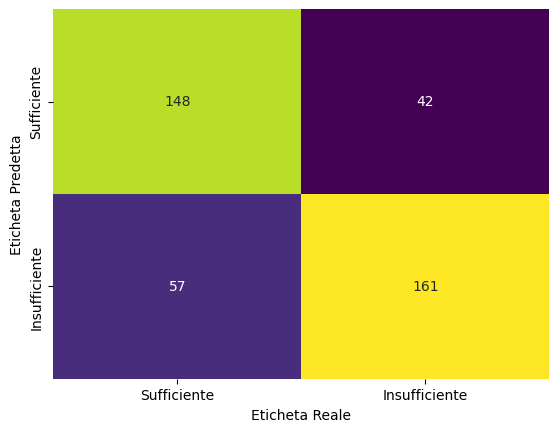
\includegraphics[width=0.6\linewidth]{confusion_matrix-GNB.png}
            \caption{  matrice di confusione Gaussian Naive Bayes}
            \label{fig:enter-label}
        \end{figure}
        \newpage
        \subsubsection{Multinomial Naive Bayes}
        L'algoritmo Multinomial Naive Bayes è la seconda variante che andremo a studiare dell'algoritmo di Naive Bayes ed è particolarmente utile per problemi di classificazione di testi\\ Notiamo la matrice di confusione disegnata:
        \begin{figure}[ht]
            \centering
            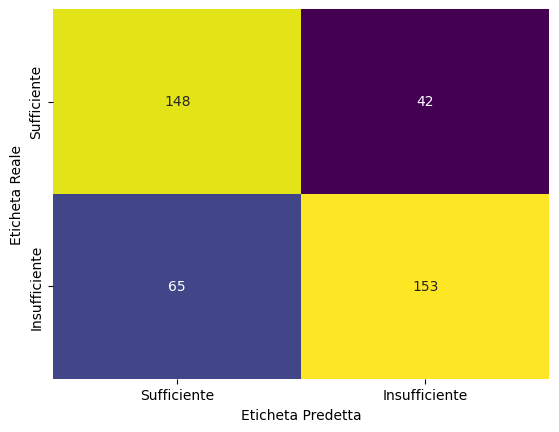
\includegraphics[width=0.6\linewidth]{confusion_matrix-MNB.png}
            \caption{  matrice di confusione Multinomial Naive Bayes}
            \label{fig:enter-label}
        \end{figure}
        
        \subsubsection{Bernoulli Naive Bayes}
        Infine, l'ultima variante che andremo a studiare è quella relativa all'algoritmo Bernoulli Naive Bayes L'algoritmo Multinomial Naive Bayes è la seconda variante che andremo a studiare dell'algoritmo di Naive Bayes ed è particolarmente utile per dati binari.
        \begin{figure}[ht]
            \centering
            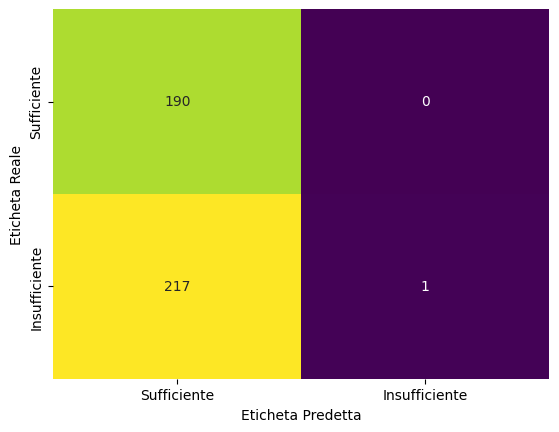
\includegraphics[width=0.6\linewidth]{confusion_matrix-BNB.png}
            \caption{  matrice di confusione Bernoulli Naive Bayes}
            \label{fig:enter-label}
        \end{figure}

        \subsubsection{Confronto tra GNB, MNB, BNB}
        Dopo aver studiato il comportamento di ogni singola variante dell'algoritmo di Naive Bayes, passiamo a confrontare i risultati ottenuti e fare le prime deduzioni. Per fare ciò ho bisogno di metriche specifiche, chiamate \textbf{metriche di valutazione}. Le principaili e quelle più famose sono \textbf{precision}, \textbf{recall} e \textbf{accuracy}; ma ho voluto studiare il comportamento anche di metriche come \textbf{F1 score} e il \textbf{MCC} (coefficiente di correlazione di Matthews):
        \begin{itemize}
            \item \textbf{Precision}: misura la proporzione di casi positivi effettivamente positivi tra tutte le predizioni positive fatte dal modello;
            \item \textbf{Recall}: misura la capacit`a del modello di identificare correttamente i casi positivi rispetto al totale dei casi positivi reali;
            \item \textbf{Accuracy}: misura la proporzione complessiva di predizioni corrette fatte dal modello rispetto al totale delle predizioni;
            \item \textbf{F1 score}: misura che viene calcolata tramite la media armonica di precision e recall;
            \item \textbf{MCC}: 
        \end{itemize}
\end{titlepage}

\end{document}
